\chapter{Simulation Results}
\textbf{Content}: Comparison of flooding to petal routing on the basis of delivery ratio, end-to-end delay, overhead, average number of hops. 
\textbf{Intent}:  Present data and analysis for the performance of petal routing.

We have used Qrsim quadrotor simulator \cite{denardi2013rn} - briefly explained in section \ref{qrsim_intro} - for evaluating our protocol. The volume of the simulated flying zone is 120 units $ \times \text{120 units} \times \text{120 units, out of which we have used 80 units} \times \text{80 units}\times $ 40 units where drones can be placed. We also have a scaling factor which scales the simulation units i.e. a scaling factor of 5 will make 1 unit in simulation to 5 meters. The drones have a reliable transmission range of $\approx 90 m$ (\fref{fig:packet_loss}) and the wi-fi antenna is omnidirectional. The simulation state changes at a time quantum of 0.2 seconds.

Initially, the drones start in a mesh formation arranged in a 2D grid as shown in \fref{fig:mesh_formation} and gradually they wrap around the plume - which, in our case, for simplicity, has been assumed to be spherical \fref{fig:final_state}. Besides these two formations, we have also evaluated our results for a random distribution of drones in the simulation space \fref{fig:random_formation}.

\begin{figure}[hbtp]
\centering
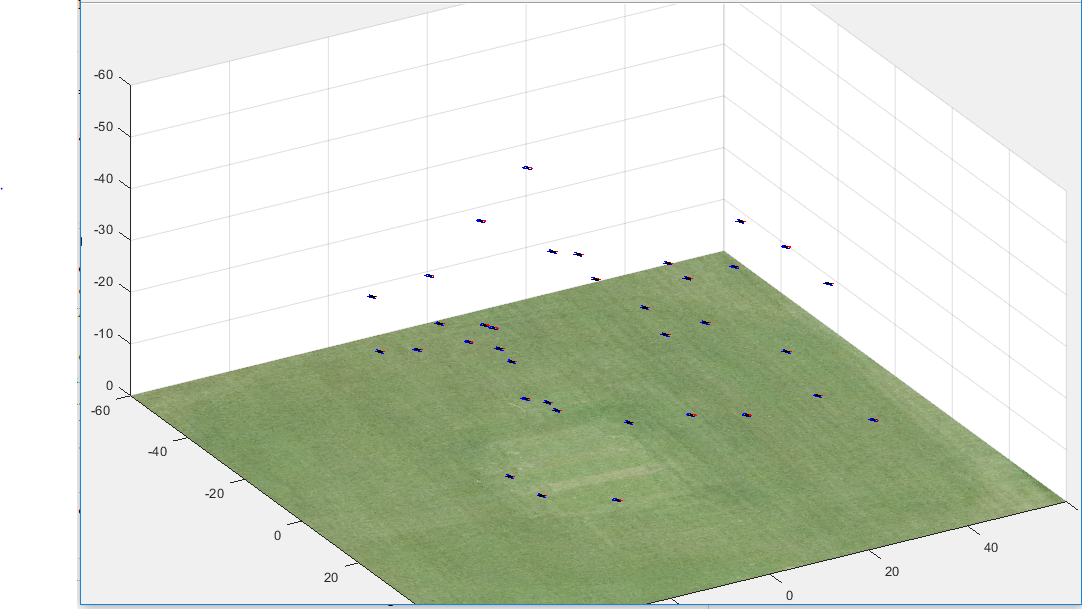
\includegraphics[width=0.8\textwidth]{ncsuthesis-0.6/Chapter-5/figs/random_drone_locations}
\caption{Random distribution of UAVs in the simulation space}
\label{fig:random_formation}
\end{figure}

The messages sent among the drones are assumed to be small and we have not considered transmission errors and congestion separately, rather they are assumed to be represented by the free space path loss model explained in section \ref{free_space_path_loss} and the parameters which are in \ref{tab:fspl_parameters}. We have picked 200 furthest pairs of drones for our result evaluation. 

In the following sections we compare the performance of our routing scheme to flooding. We shall be studying the following performance metrics `Packet delivery ratio', `Average end-to-end delay', `Average number of hops', `Average number of transmissions' \cite{OUBBATI201729}:

We compare these metrics for three arrangements of the UAVs namely, \emph{mesh} - \fref{fig:mesh_formation}, \emph{random} - \fref{fig:random_formation}, \emph{spherical} - \fref{fig:final_state}. The three formations have peculiar properties, for example the spherical formation has the plume acting as a \emph{routing void}, whereas the mesh formation represents a 2D formation and thus we can study the performance of our 3D routing scheme in a 2D setting. Finally, random placement of the drones lets us study the performance in a generic situation.

\section{Packet delivery ratio}
\label{pdr}
    \textbf{Packet delivery ratio (PDR):} is defined as the ratio of `count of all packets successfully delivered ($P_r$)' to `count of all the packets transmitted by the sender (P)'. PDR characterizes the robustness and reliability of a routing scheme. The bigger is PDR, the better is the performance of the protocol. 
\begin{figure}[hbtp]
\centering
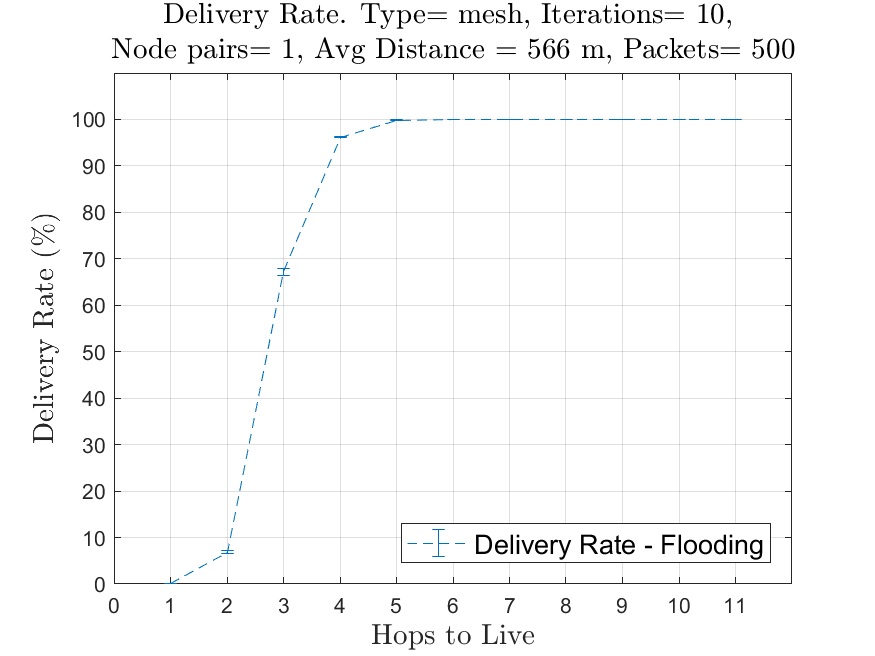
\includegraphics[width=1\textwidth]{ncsuthesis-0.6/Chapter-5/figs/fl_DR_mesh.png}
\caption{Delivery rate in mesh formation for flooding}
\label{fig:fl_DR_mesh}
\end{figure}

\begin{figure}[hbtp]
\centering
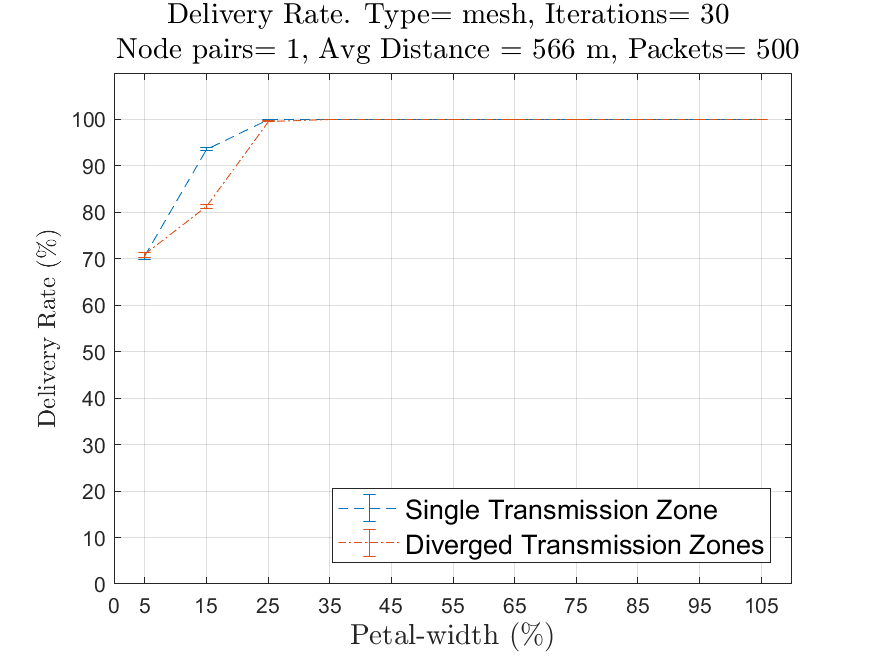
\includegraphics[width=1\textwidth]{ncsuthesis-0.6/Chapter-5/figs/pe_DR_mesh.png}
\caption{Delivery rate in mesh formation}
\label{fig:pe_DR_mesh}
\end{figure}

\begin{figure}[hbtp]
\centering
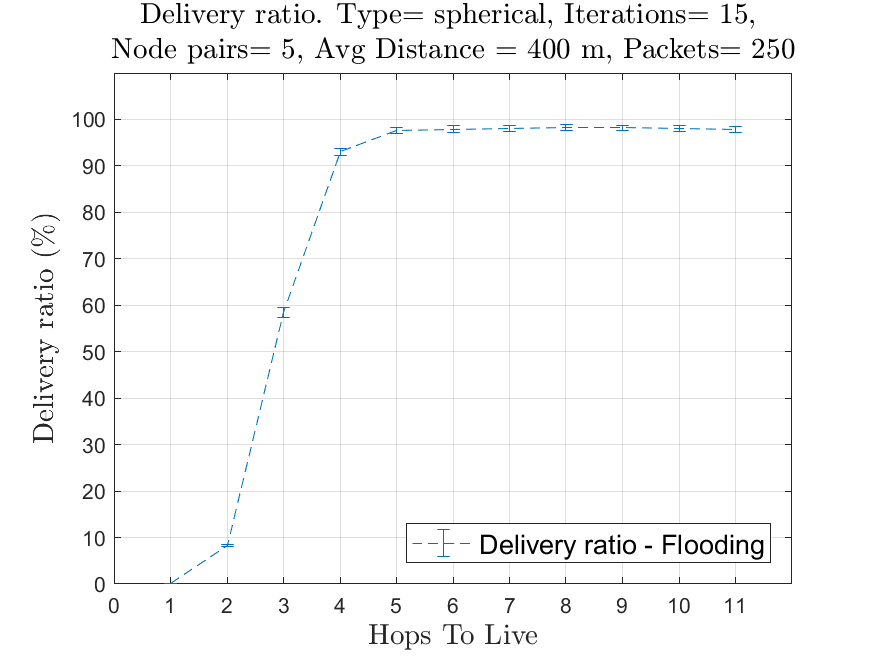
\includegraphics[width=1\textwidth]{ncsuthesis-0.6/Chapter-5/figs/fl_DR_spherical.png}
\caption{Delivery rate in spherical formation for flooding}
\label{fig:fl_DR_spherical}
\end{figure}

\begin{figure}[hbtp]
\centering
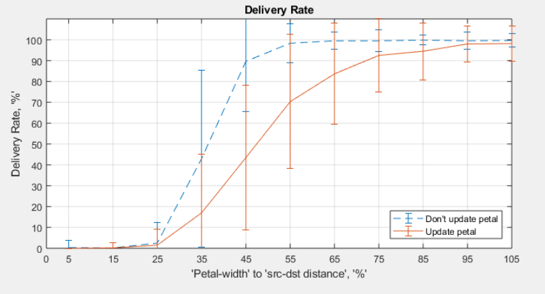
\includegraphics[width=1\textwidth]{ncsuthesis-0.6/Chapter-5/figs/pe_DR_spherical.png}
\caption{Delivery rate in spherical formation}
\label{fig:pe_DR_spherical}
\end{figure}

\begin{figure}[hbtp]
\centering
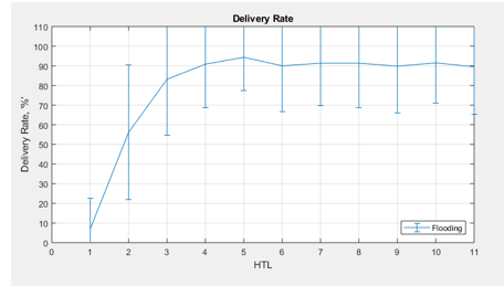
\includegraphics[width=1\textwidth]{ncsuthesis-0.6/Chapter-5/figs/fl_DR_random.png}
\caption{Delivery rate in random formation for flooding}
\label{fig:fl_DR_random}
\end{figure}

\begin{figure}[hbtp]
\centering
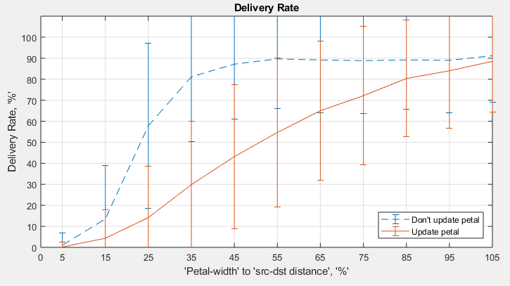
\includegraphics[width=1\textwidth]{ncsuthesis-0.6/Chapter-5/figs/pe_DR_random.png}
\caption{Delivery rate in random formation}
\label{fig:pe_DR_random}
\end{figure}

\fref{fig:fl_DR_mesh} shows a plot of PDR vs HTL of the packets sent. It should be noted that for small HTL values (e.g. HTL = 1) the PDR is low because the intermediate nodes don't forward the packets. However as HTL approaches the diameter of the network PDR approaches 90\% delivery rate which is an upperbound for the PDR of any routing algorithm. \fref{fig:pe_DR_mesh} shows the PDR of our protocol which approaches the PDR of flooding algorithm at 15\% width.

\section{Average end-to-end delay}
    \textbf{Average end-to-end delay (EED):} is defined as the average time for data packets to reach the target destinations. Only the data packets successfully received and generated are counted. The smaller is EED, the better is the performance of the protocol.
    
\begin{figure}[hbtp]
\centering
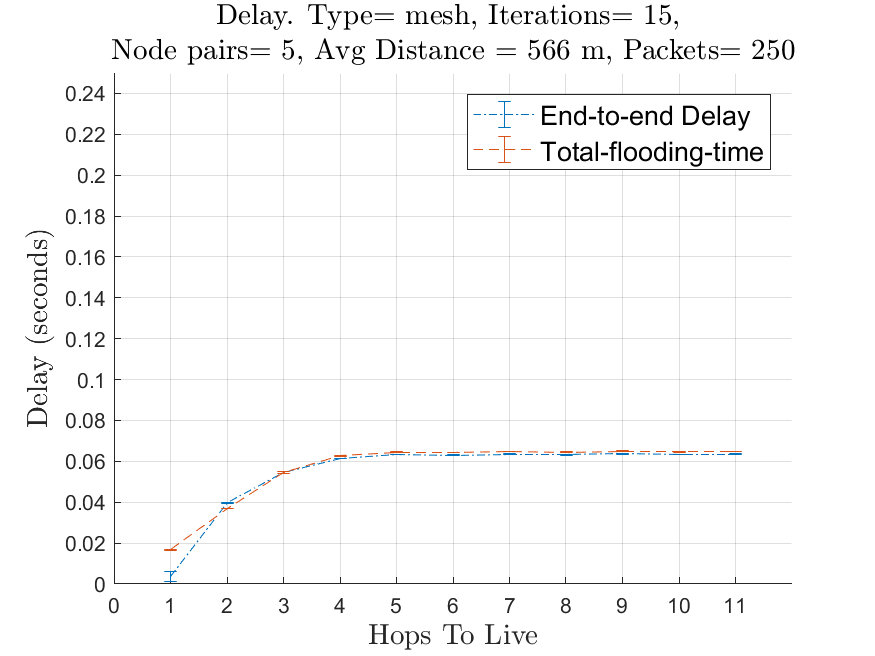
\includegraphics[width=1\textwidth]{ncsuthesis-0.6/Chapter-5/figs/fl_delay_mesh.png}
\caption{End-to-end delay in mesh formation for flooding}
\label{fig:fl_delay_mesh}
\end{figure}

\begin{figure}[hbtp]
\centering
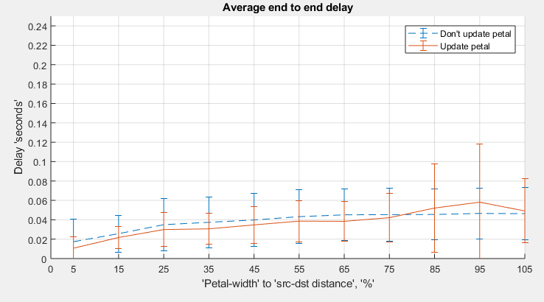
\includegraphics[width=1\textwidth]{ncsuthesis-0.6/Chapter-5/figs/pe_delay_mesh.png}
\caption{End-to-end delay in mesh formation}
\label{fig:pe_delay_mesh}
\end{figure}

\begin{figure}[hbtp]
\centering
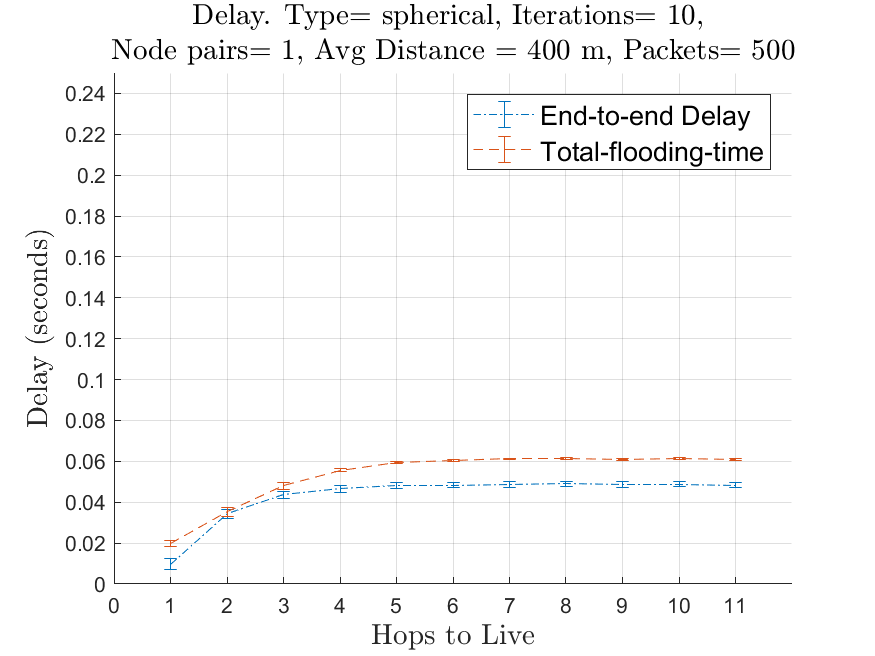
\includegraphics[width=1\textwidth]{ncsuthesis-0.6/Chapter-5/figs/fl_delay_spherical.png}
\caption{End-to-end delay in spherical formation for flooding}
\label{fig:fl_delay_spherical}
\end{figure}

\begin{figure}[hbtp]
\centering
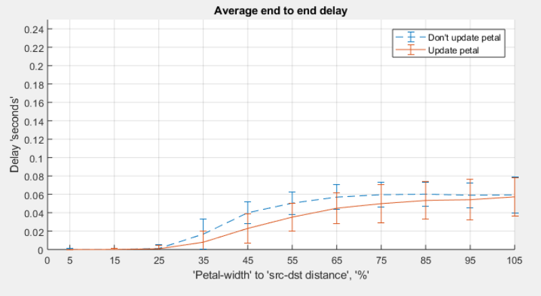
\includegraphics[width=1\textwidth]{ncsuthesis-0.6/Chapter-5/figs/pe_delay_spherical.png}
\caption{End-to-end delay in spherical formation}
\label{fig:pe_delay_spherical}
\end{figure}

\begin{figure}[hbtp]
\centering
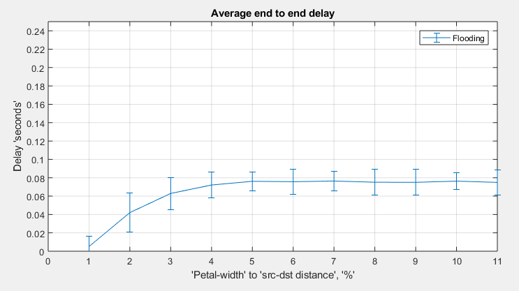
\includegraphics[width=1\textwidth]{ncsuthesis-0.6/Chapter-5/figs/fl_delay_random.png}
\caption{End-to-end delay in random formation for flooding}
\label{fig:fl_delay_random}
\end{figure}

\begin{figure}[hbtp]
\centering
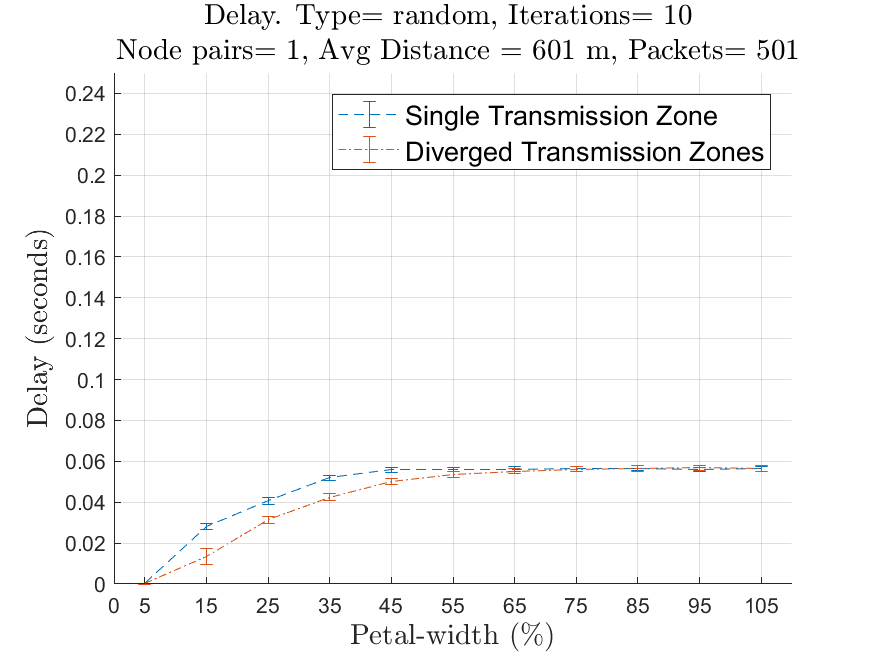
\includegraphics[width=1\textwidth]{ncsuthesis-0.6/Chapter-5/figs/pe_delay_random.png}
\caption{End-to-end delay in random formation}
\label{fig:pe_delay_random}
\end{figure}

End-to-end delay characterizes the tolerable delay in the network. The EED should be as low as possible to support real-time traffic. This metric is more important in UAV missions like live survellience or disaster monitoring. \fref{fig:fl_delay_mesh} plots the EED vs HTl and \fref{fig:pe_delay_mesh} plots the EED for our routing algorithm. Applications that require real-time visual or audio data transfers, a delay of 50-100 ms is acceptable. As such both the algorithms fulfill this requirement, however our protocol has an EED of $\le 40 ms$ and is always lower than flooding.

\section{Average number of hops}
    \textbf{Average number of hops (H):} is defined as the number of data packets delivered divided by the number of hops performed by all packets. Consumption of resources is proportional to the average number of hops. The smaller is `H' the better is the protocol.

\begin{figure}[hbtp]
\centering
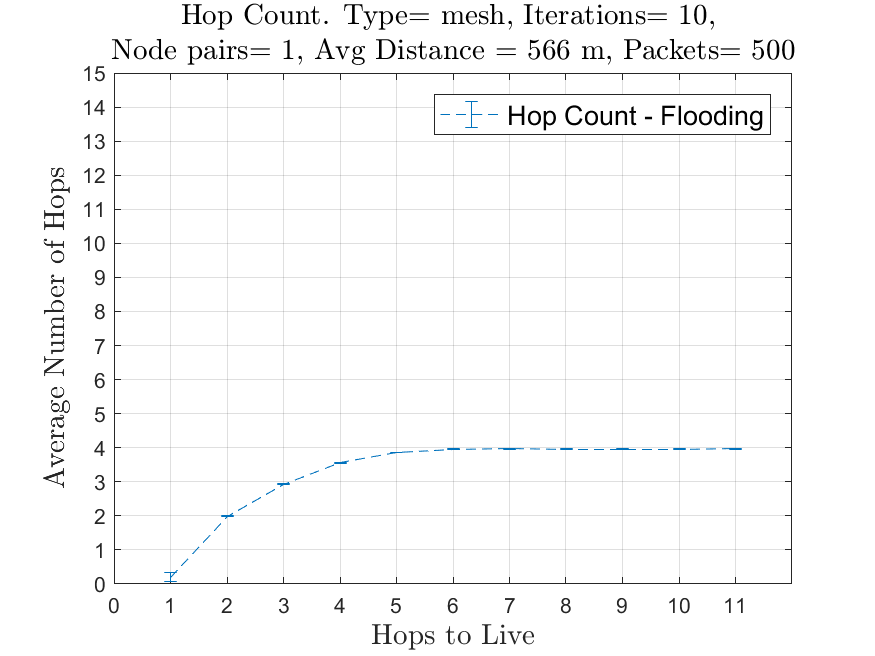
\includegraphics[width=1\textwidth]{ncsuthesis-0.6/Chapter-5/figs/fl_hops_mesh.png}
\caption{Number of hops: mesh formation, flooding algorithm}
\label{fig:fl_hops_mesh}
\end{figure}

\begin{figure}[hbtp]
\centering
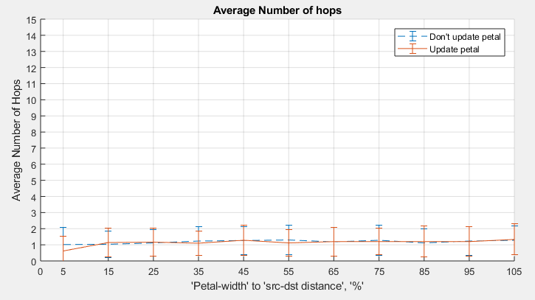
\includegraphics[width=1\textwidth]{ncsuthesis-0.6/Chapter-5/figs/pe_hops_mesh.png}
\caption{Number of hops: mesh formation}
\label{fig:pe_hops_mesh}
\end{figure}

\begin{figure}[hbtp]
\centering
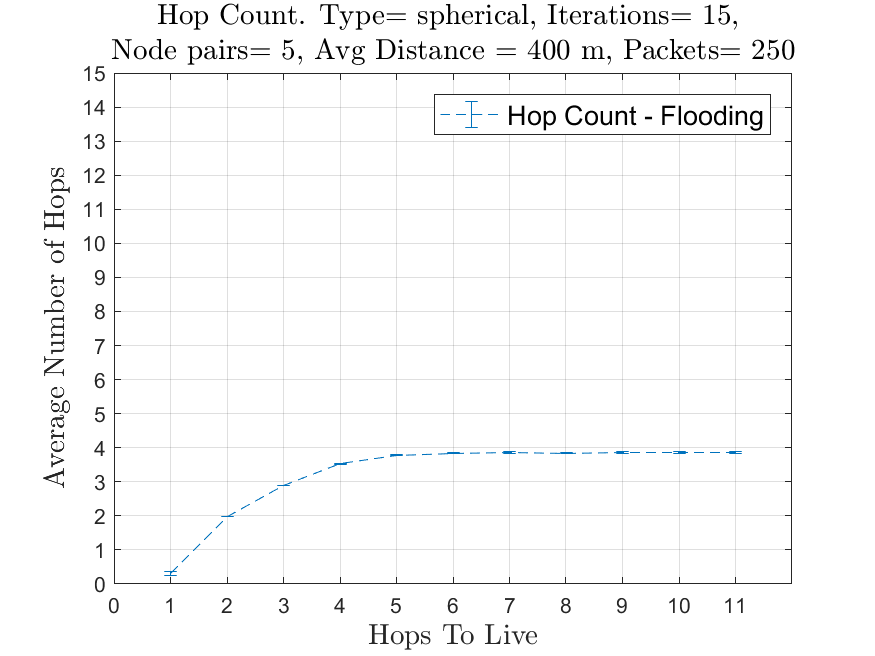
\includegraphics[width=1\textwidth]{ncsuthesis-0.6/Chapter-5/figs/fl_hops_spherical.png}
\caption{Number of hops: spherical formation, flooding algorithm}
\label{fig:fl_hops_spherical}
\end{figure}

\begin{figure}[hbtp]
\centering
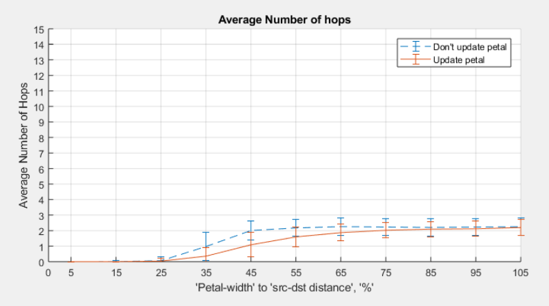
\includegraphics[width=0.9\textwidth,height=0.9\textheight,keepaspectratio]{ncsuthesis-0.6/Chapter-5/figs/pe_hops_spherical.png}
\caption{Number of hops: spherical formation}
\label{fig:pe_hops_spherical}
\end{figure}

\begin{figure}[hbtp]
\centering
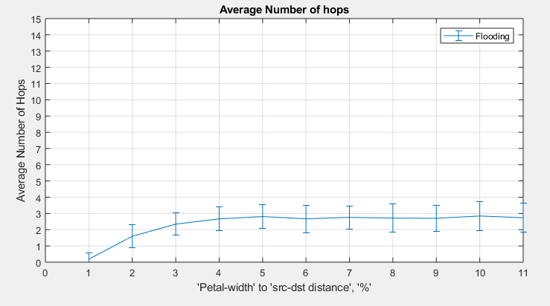
\includegraphics[width=0.9\textwidth,height=0.9\textheight,keepaspectratio]{ncsuthesis-0.6/Chapter-5/figs/fl_hop_random.png}
\caption{Number of hops: mesh formation, flooding algorithm}
\label{fig:fl_hops_random}
\end{figure}

\begin{figure}[hbtp]
\centering
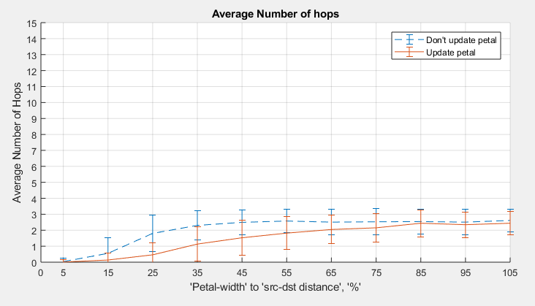
\includegraphics[width=\textwidth,height=\textheight,keepaspectratio]{ncsuthesis-0.6/Chapter-5/figs/pe_hop_random.png}
\caption{Number of hops: mesh formation}
\label{fig:pe_hops_random}
\end{figure}


The number of hops a packet makes before reaching the destination is a representation of the resources consumed in delivering the packet. With antennas having fixed transmitting strength, reducing the number of hops reduces the energy expenditure. \fref{fig:fl_hops_mesh} plots the average number of hops for flooding and \fref{fig:pe_hops_mesh} plots the average number of hops for our routing scheme.

\section{Average number of transmission}
    \textbf{Average number of transmissions (NT):} is defined as the total number of transmissions divided by the total number packets successfully delivered. In an ideal routing protocol `NT' would be equal to H $\times$ `number of packets delivered'. The lower is `NT', the better is the protocol. 
    
\begin{figure}[hbtp]
\centering
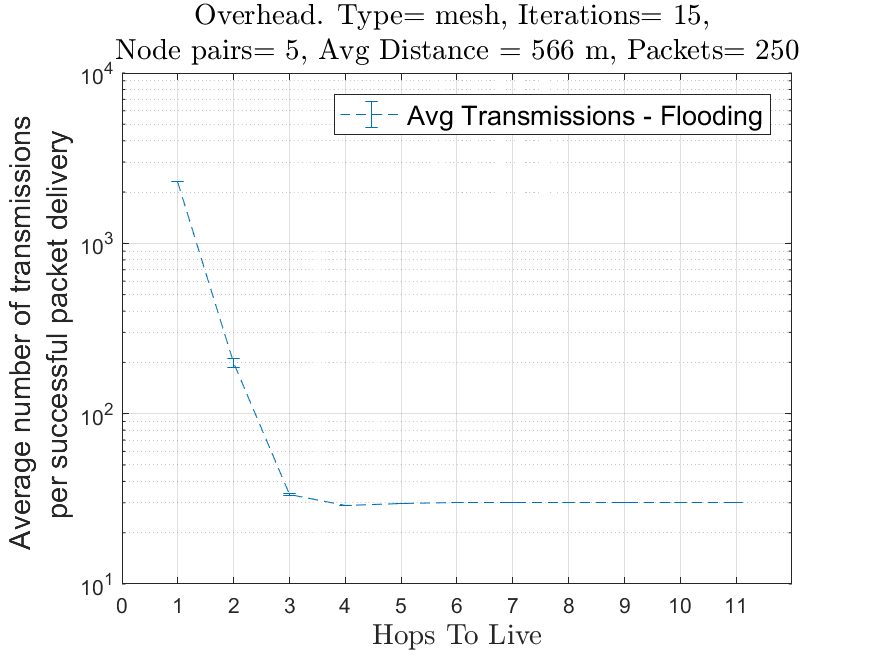
\includegraphics[width=\textwidth,height=\textheight,keepaspectratio]{ncsuthesis-0.6/Chapter-5/figs/fl_trans_mesh.png}
\caption{Number of transmissions: mesh formation, flooding algorithm}
\label{fig:fl_trans_mesh}
\end{figure}

\begin{figure}[hbtp]
\centering
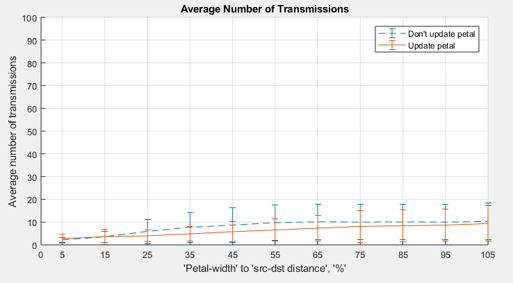
\includegraphics[width=\textwidth,height=\textheight,keepaspectratio]{ncsuthesis-0.6/Chapter-5/figs/pe_trans_mesh.png}
\caption{Number of transmissions: mesh formation}
\label{fig:pe_trans_mesh}
\end{figure}

\begin{figure}[hbtp]
\centering
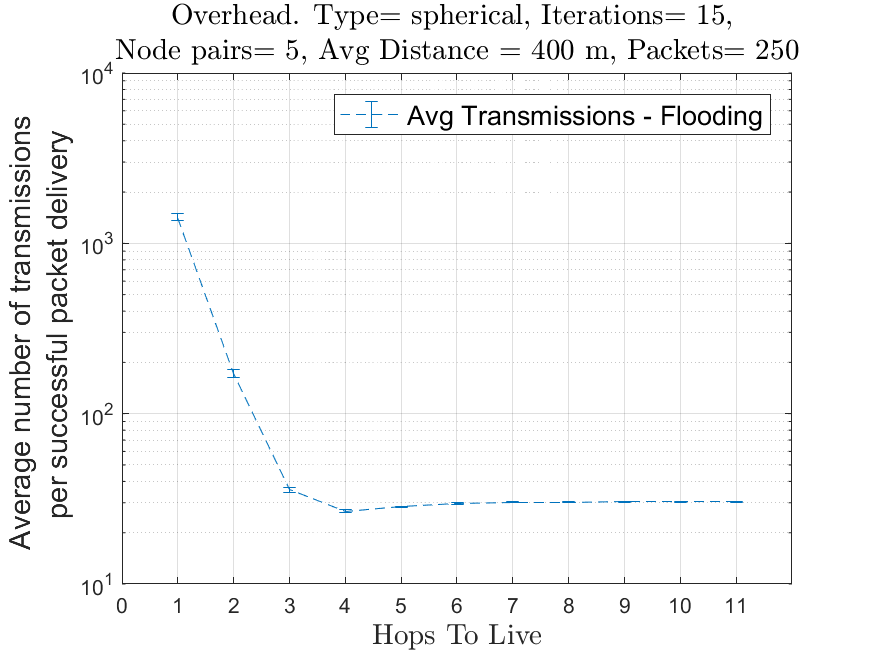
\includegraphics[width=\textwidth,height=\textheight,keepaspectratio]{ncsuthesis-0.6/Chapter-5/figs/fl_trans_spherical.png}
\caption{Number of transmissions: spherical formation, flooding algorithm}
\label{fig:fl_trans_spherical}
\end{figure}

\begin{figure}[hbtp]
\centering
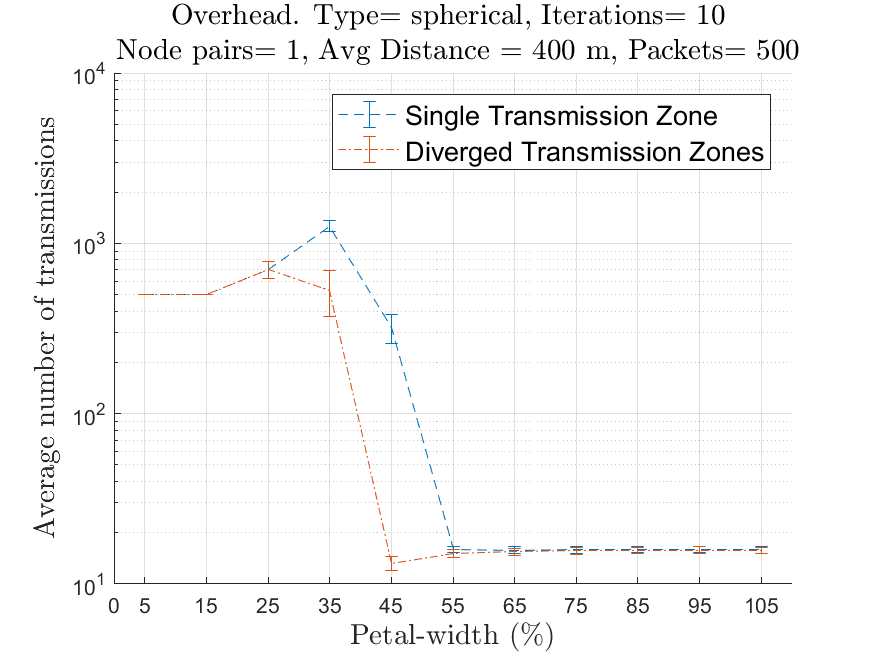
\includegraphics[width=\textwidth,height=\textheight,keepaspectratio]{ncsuthesis-0.6/Chapter-5/figs/pe_trans_spherical.png}
\caption{Number of transmissions: spherical formation}
\label{fig:pe_trans_spherical}
\end{figure}

\begin{figure}[hbtp]
\centering
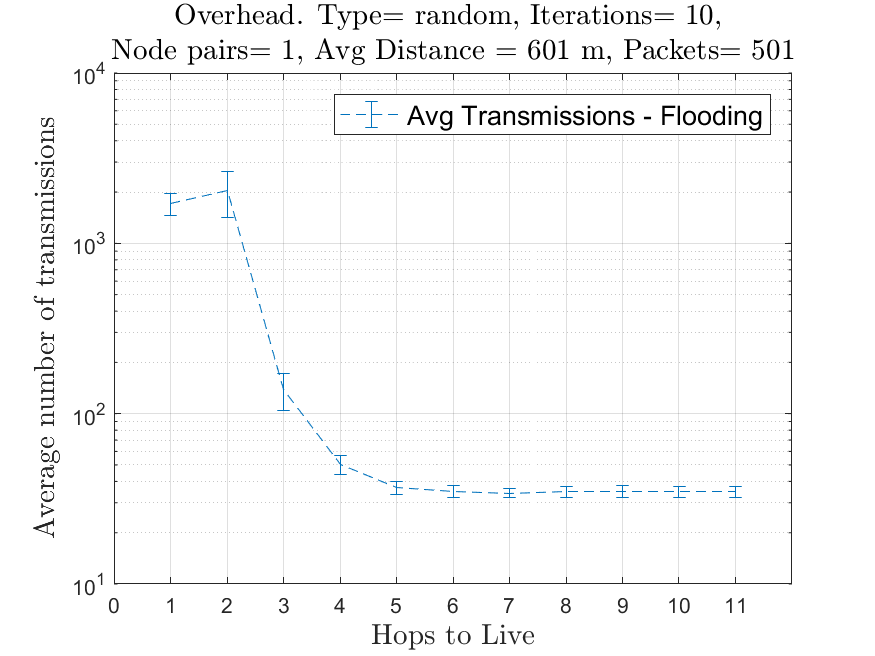
\includegraphics[width=\textwidth,height=\textheight,keepaspectratio]{ncsuthesis-0.6/Chapter-5/figs/fl_trans_random.png}
\caption{Number of transmissions: random formation, flooding algorithm}
\label{fig:fl_trans_random}
\end{figure}

\begin{figure}[hbtp]
\centering
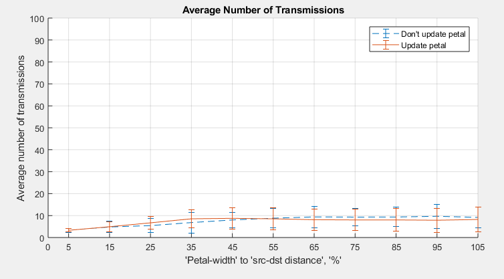
\includegraphics[width=\textwidth,height=\textheight,keepaspectratio]{ncsuthesis-0.6/Chapter-5/figs/pe_tran_random.png}
\caption{Number of transmissions: random formation}
\label{fig:pe_trans_random}
\end{figure}

Number of transmissions is the combined transmissions from all nodes for each successful packet delivery. `NT' directly influences the energy spent in routing a packet. For a successfully delivered packet the upper bound of `NT' is the total number of nodes in the network. This can be noticed for flooding algorithm in \fref{fig:fl_trans_mesh} where NT is approximately equal to the total number of nodes, whereas in our routing algorithm (\fref{fig:pe_trans_mesh}) the number of transmissions drops significantly due to the restricted flooding approach.

\section{Effect of network density}

\begin{figure}[hbtp]
\centering
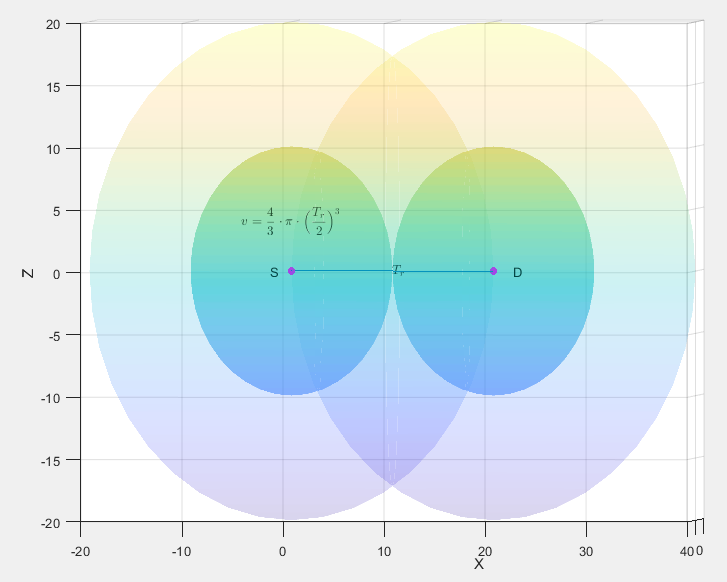
\includegraphics[width=1\textwidth]{ncsuthesis-0.6/Chapter-5/figs/nodeDensity}
\caption{Ideal network density}
\label{fig:node_density}
\end{figure}

\textbf{Node density:} Assuming that a perfectly omnidirectional antenna can deliver packets directly and reliably to a receiver at a distance of `r' meter  in space; the volume covered by the transmitter would be $ v = \dfrac{4}{3} \cdot \pi \cdot \Big( \dfrac{T_r}{2}\big)^3 $. In \fref{fig:node_density}, the bigger spheres represent the reach of a transmitter and the smaller spheres represent the ideal separation of two neighboring antennas. Considering the volume of the flying space is V, and the number of drones in the space is DC, we classify the node density of the simulation as sparse, ideal and high according to the following relation.

\begin{eqnarray} \label{node_density}
\begin{aligned}
& \text{Sparse node density:} & \dfrac{V}{v} << DC \\
& \text{Ideal node density:} & \dfrac{V}{v} \approx DC \\
& \text{High node density:} & \dfrac{V}{v} >> DC
\end{aligned}
\end{eqnarray}

For example, with scaling factor = 4, Number of Drones = 36, and flying space volume = $ 80 \times 80 \times 40 unit^3  \text{and } T_r = 90 m $,
\begin{eqnarray*}
& \text{we have,} & V = 80 \times 80 \times 40 \times 64 = 16384000 unit^3 \\
& {and} & v = \dfrac{4 \times 3.14 \times (\frac{90}{2}) ^ 3}{3} \approx 381510 unit ^ 3 \\
& \Rightarrow idealDroneCount = & \dfrac{V}{v} \approx 43
\end{eqnarray*}

Since, the number of drones in our simulation (36) is close to \emph{idealDroneCount}, the metrics we presented in the previous sections were for ideal network density. In this section we shall study the effect of network density on the performance our routing scheme and flooding.

As we observed in section \ref{pdr}, the PDR for flooding algorithm depends on the HTL and is $>90\%$ for $HTL>4$ whereas PDR depends on petal width in case of petal routing and $>90\%$ for $width>35\%$. 
Therefore, to study the effects of network density we have picked HTL = 10 for flooding and petal width = 35\% for petal routing. 

\begin{figure}[hbtp]
\centering
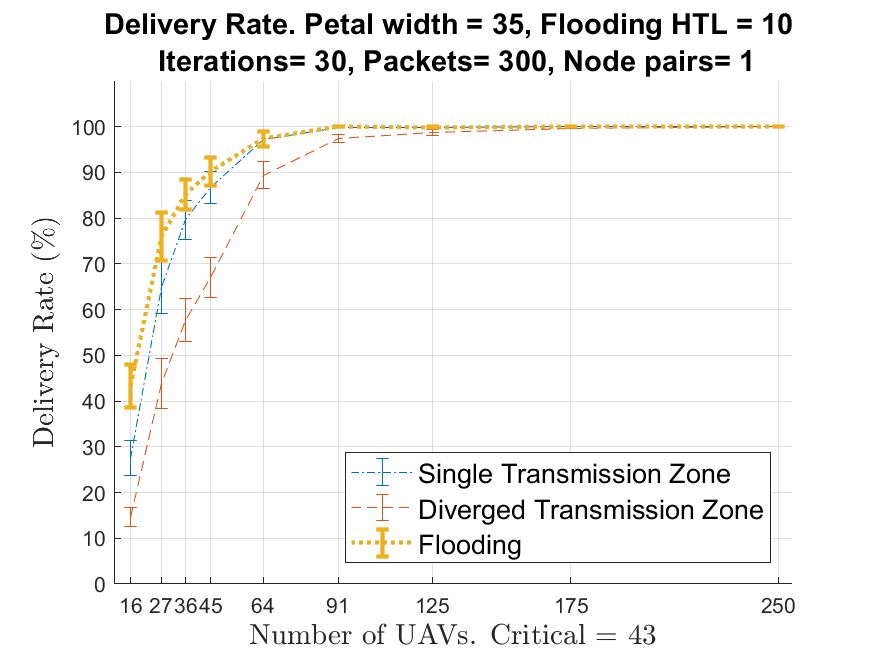
\includegraphics[width=1\textwidth]{ncsuthesis-0.6/Chapter-5/figs/ND_DR}
\caption{Delivery rate vs network density}
\label{fig:nd_DR}
\end{figure}

\fref{fig:nd_DR} shows the variation in delivery ratio vs network density. We can observe that the PDR for flooding is higher in sparse network density as compared to petal routing. This is expected because there might not be sufficient intermediate nodes to forward the packet towards destination. However, as expected PDR for petal routing approaches that of flooding when the network density is close to the ideal network density. Specifically, the PDR is $ > 90\%$ when number of UAVs is higher than 36.

\begin{figure}[hbtp]
\centering
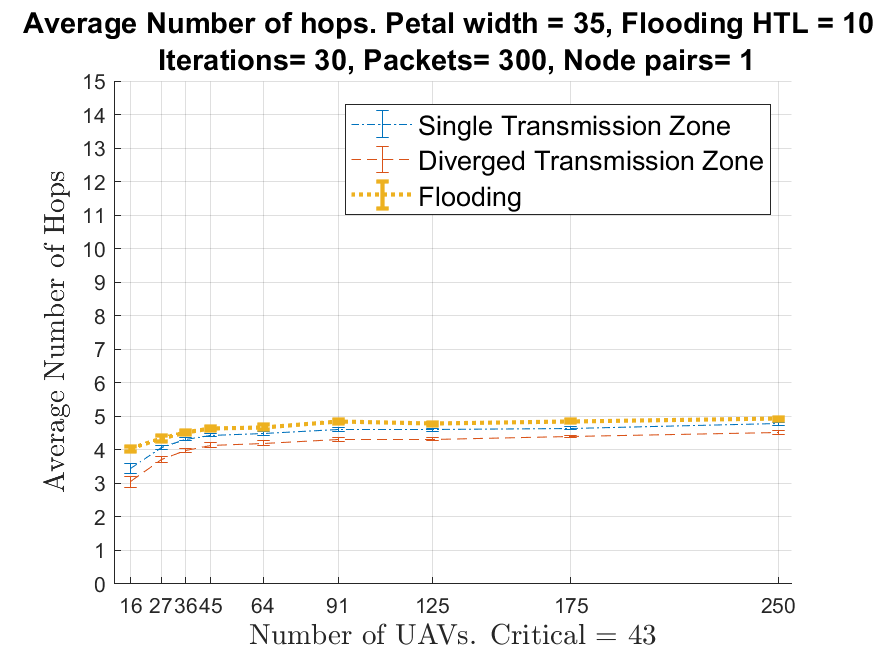
\includegraphics[width=1\textwidth]{ncsuthesis-0.6/Chapter-5/figs/ND_hops}
\caption{Average number of hops vs network density}
\label{fig:ND_hops}
\end{figure}

\fref{fig:ND_hops} depicts the change in average number of hops as compared to the network density. We can observe that the number of hops doesn't vary much with increase in network density. This is also expected since in both the algorithms the packets propagate in a breadth first manner and hence find the shortest path to the destination. 

\begin{figure}[hbtp]
\centering
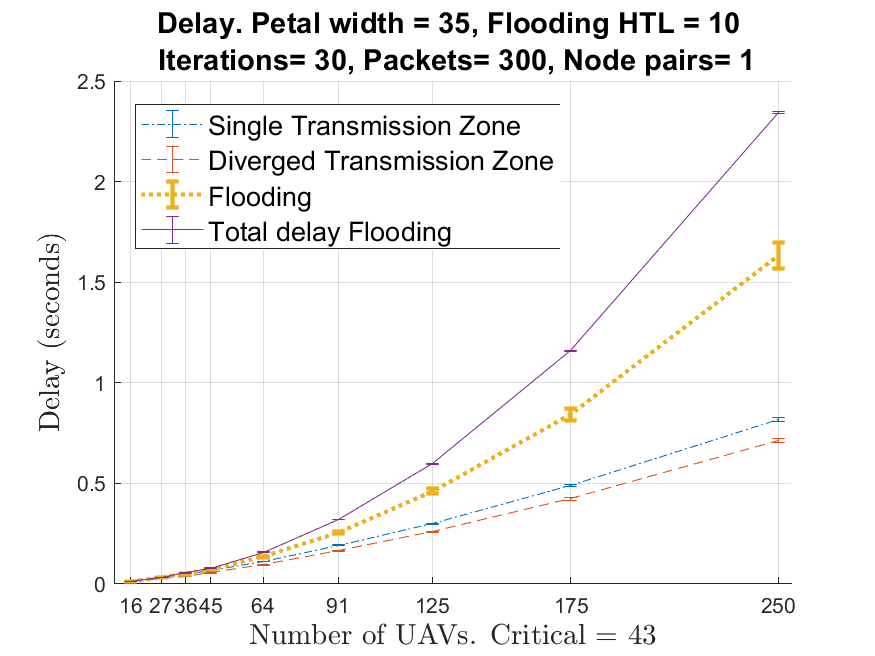
\includegraphics[width=1\textwidth]{ncsuthesis-0.6/Chapter-5/figs/ND_delay}
\caption{End-to-end delay vs network density}
\label{fig:ND_delay}
\end{figure}

In \fref{fig:ND_delay}, we can observe the change in end-to-end delay with network density. The rate of increase in end-to-end delay for flooding is higher than that of petal routing which is due to the excessive number of retransmissions in the network. Since, our routing algorithm restricts the transmissions to a zone thereby pruning the unnecessary retransmissions.  

\begin{figure}[hbtp]
\centering
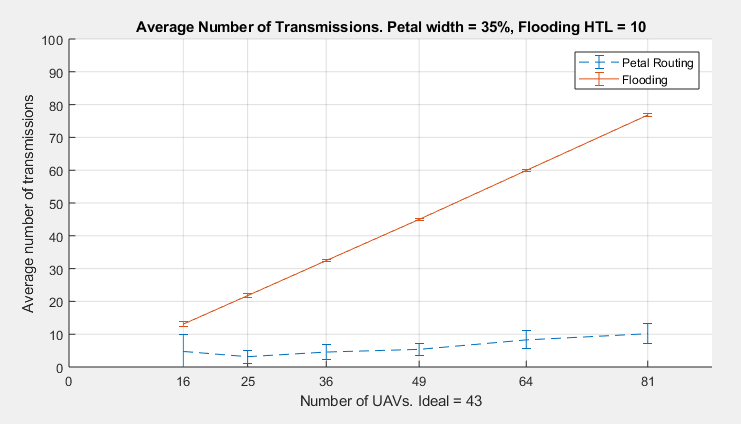
\includegraphics[width=1\textwidth]{ncsuthesis-0.6/Chapter-5/figs/ND_trans}
\caption{Average number of transmission vs network density}
\label{fig:ND_trans}
\end{figure}

In \fref{fig:ND_trans} we observe that the average number of transmissions increases with increase in network density. However, the increase is more steep for flooding algorithm as compared to petal routing. Specifically, for flooding algorithm, the average number of transmissions is roughly equal to the number of nodes in the network. This is expected since all the nodes which receive a packet transmit at least once in case of flooding; however, in our routing scheme we restrict the retransmissions to a zone and by back-off mechanism as well.

\section{Discussions}

Our routing algorithm doesn't maintain or exchange any topology graph hence it neither needs to exchange control information nor it has to do the computation heavy path calculations.

Moreover, our algorithm doesn't do a route discovery, which eliminates the typical delay associated with reactive routing algorithms. 

Our algorithm is robust i.e. the messages are routed through geo-diffuse pathsets and matches the delivery rate of flooding.

These are the expectations of a routing algorithm that would be suitable for our mission. 
\begin{enumerate}
\item Packet delivery rate between any two pairs of nodes should be approximately equal to a flooding algorithm. 
\item The average number of total transmission per transmitted packet should be significantly lower than flooding.
\end{enumerate}
